\documentclass[]{beamer}
% \geometry{papersize={16cm,9.60cm}}
\usepackage{etex}
\usepackage{amsmath}
\usepackage{tikz}
\usepackage{multimedia}
\usetheme{Boadilla}
\usepackage{graphicx}
\usepackage{url}

%\usepackage{inputenc}

% \mode<presentation>
% {
%   \usetheme{default}
%   \setbeamercovered{transparent}
% }


% {\vskip5pt}

%% customize layout, bullet points navigation toolbar
\setbeamertemplate{navigation symbols}{}%remove navigation symbols
\setbeamertemplate{enumerate items}[default]
\setbeamertemplate{navigation symbols}{}
\setbeamertemplate{itemize items}[circle]
\setbeamercolor{enumerate item}{fg=black}

\setbeamertemplate{footline}{}
\setbeamersize{text margin left = 2.0em}
\setbeamersize{text margin right = 2.0em}


\usepackage{times}
\usepackage[T1]{fontenc}

% Or whatever. Note that the encoding and the font should match. If T1
% does not look nice, try deleting the line with the fontenc.

\setbeamertemplate{navigation symbols}{}

\title{ Cognitive (Neuro) Psychology }
\subtitle{IX. Reaching and grasping}
\author{ Marianne Maertens }
\institute[TU Berlin]{Technische Universit\"at Berlin}
\date{September 2016}

\begin{document}
\setbeamertemplate{enumerate items}[default]
\setbeamertemplate{headline}

\frame{\titlepage}

\AtBeginSection[]
{
  \begin{frame}<beamer>
    \frametitle{Layout}
    \tableofcontents[currentsection]
  \end{frame}
}

\begin{frame}
 \frametitle{Hands}
\begin{overlayarea}{130mm}{80mm}
Manual performance is central to human experience
\begin{columns}[T]
 \begin{column}{40mm}
\begin{center}
\begin{itemize}
 \item build houses
 \item draw pictures
 \item make bread
 \item play instruments
 \item gesture
\end{itemize}
\end{center}
 \end{column}
 \begin{column}{80mm}

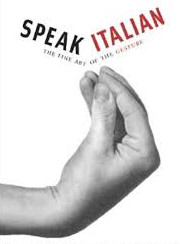
\includegraphics[width=30mm]{figs/l9/italian_gesture.jpg}
 \end{column}
\end{columns}

\only<3->{
\vspace{5mm}
``one the one hand and on the other''\\
``ideas go hand in hand''\\
``an offhand remark''}
\end{overlayarea}
 \end{frame}


\begin{frame}
\frametitle{Reaching and Grasping}
 
 \begin{center}
\includegraphics<1>[width=100mm]{figs/l9/grasping_overview.png}
 \end{center}

reaching and grasping depend on a blend of initial planning and subsequent correction
\end{frame}


\begin{frame}
 \frametitle{Outline}
\begin{itemize}[<+->]
  \setlength{\itemsep}{5pt}
 \item Development of Reaching and Grasping
 \item Visual Guidance
 \item Aiming
 \item 
\end{itemize}
\end{frame}


\begin{frame}
 \frametitle{The development of reaching and grasping}
\begin{overlayarea}{110mm}{85mm}
\begin{columns}[T]
 \begin{column}{25mm}
\begin{center}
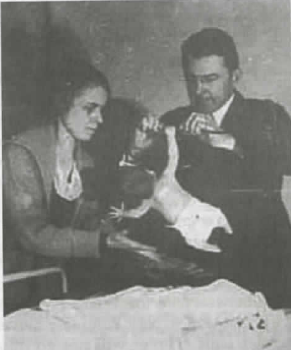
\includegraphics[width=30mm]{figs/l9/grasp_reflex.png}
\end{center}
 \end{column}
 \begin{column}{80mm}
  \begin{itemize}
   \item \textbf{grasp reflex} - infants automatically hold an object placed in their hands, disappears by around 6 months of age 
 \item<2-> \textbf{distance control} - identify distances over which infants are willing or unwilling to reach, 4-5months 
 \begin{itemize}
 \item<3-> interesting object out of reach - refrain from reaching for it
 \item<3->if distances that elicit reaches are sharply demarcated from distances that do not elicit reaches, and the boundary between the two approximates infant's arm length
 \item<3->[$\rightarrow$] infant perceives distances veridically and has information about arm length
 \end{itemize}
\item<4-> \textbf{size control} - preprogrammed grip aperture based on visual information, >9months
  \end{itemize}
 \end{column}
\end{columns}
\end{overlayarea}
\end{frame}


\begin{frame}
 \frametitle{Functional tuning of grasps in infancy}
\begin{overlayarea}{110mm}{80mm}

\begin{center}
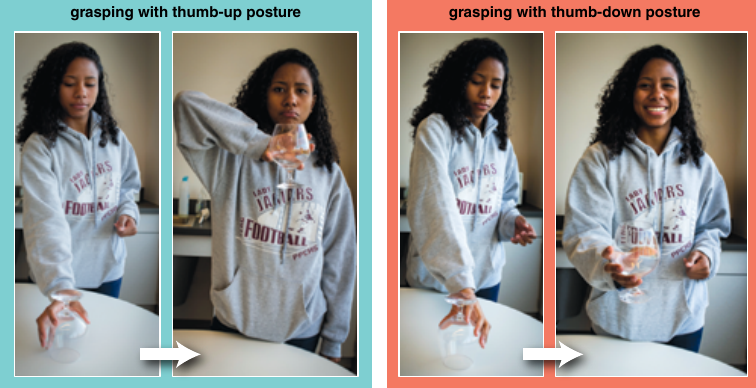
\includegraphics[width=60mm]{figs/l9/grasp_planning.png}
\end{center}
\begin{itemize}
 \item<2-> infants alter the way they reach for and grasp objects depending on what they \textbf{plan} to do with the object > 19-24months
 \item<3-> \textbf{anticipatory planning} interesting from a cognitive psychologist's point of view - reflect mental representations
 \item<4-> mental representations likely to underlie tool use - purposeful use of a tool for a goal - comparison of anticipatory strategies in infants and monkeys informative for theories of tool development
\end{itemize}
\end{overlayarea}
\end{frame}

\begin{frame}
 \frametitle{Visual Guidance}
\begin{overlayarea}{120mm}{90mm}
\begin{itemize}
 \item reaching for a seen object benefits from visual feedback
 \item reaching suffers when eyes are closed
 \item[$\rightarrow$] How is vision used in the control of reaches and grasps?
\end{itemize}

\begin{center}
\includegraphics<1>[width=50mm]{figs/l9/visual_guidance.png}
\includegraphics<2->[width=90mm]{figs/l9/soma_setup.png}

\includegraphics<3>[width=50mm]{figs/l9/rbo_traces_blurred.png}
\end{center}
\end{overlayarea}
\end{frame}

\begin{frame}
 \frametitle{Visual Guidance}
\begin{overlayarea}{120mm}{90mm}

\begin{columns}[T]
 \begin{column}{20mm}
\begin{center}
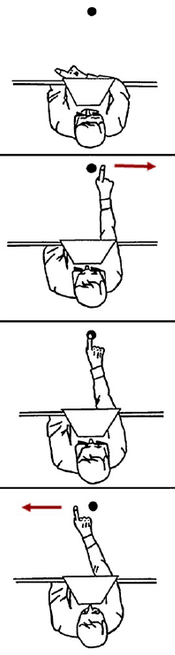
\includegraphics[width=20mm]{figs/l9/phases_prism_adaptation_images.png}
\end{center}
 \end{column}
 \begin{column}{90mm}
 \begin{center}
    \begin{itemize}
   \item adults can adjust reaching behavior based on exposure to new visual conditions (Stratton, 1897) 
 \item<2-> perceptual-motor coordination is plastic
 \item<3-> adaptation to lenses because of
 \begin{itemize}
  \item new correlation between vision and proprioception
  \item new correlation between vision and actively generated motor commands
 \end{itemize}
 \item<4-> active movement, passive movement and observation group - only active movement group learned 
  \end{itemize}
\end{center} 
\end{column}
\end{columns}
\end{overlayarea}
\end{frame}


\begin{frame}
 \frametitle{Vision and Touch}
\begin{overlayarea}{120mm}{90mm}
\begin{itemize}
 \item learning new correlations between the way things feel and look 
 \item[$\rightarrow$] does vision change, does touch change, or both?
\end{itemize}

\begin{center}
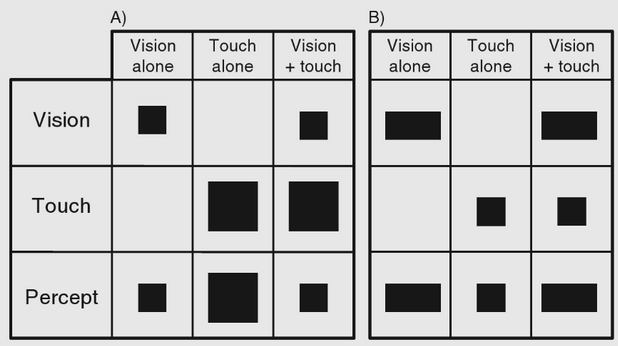
\includegraphics[width=70mm]{figs/l9/rock_harris_67.png}
\end{center}
\begin{itemize}
 \item<2-> vision dominated touch (Rock and Harris, 1967)
 \item<3-> vision less alerting than touch $\rightarrow$ more voluntary attention on vision
\end{itemize}

\end{overlayarea}
\end{frame}


\begin{frame}
 \frametitle{Vision for Action}
\begin{overlayarea}{120mm}{90mm}
 \begin{itemize}
 \item same perception if one is looking at a scene for the sake of recognizing objects or for the sake of acting
 \end{itemize}

\begin{center}
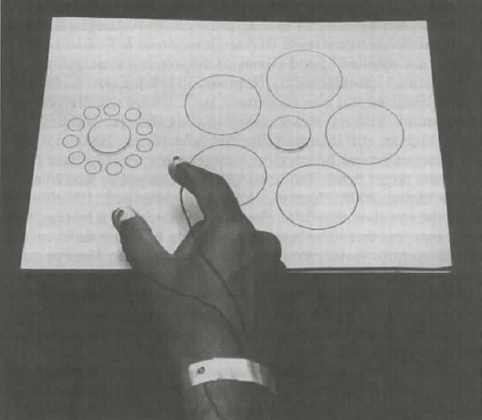
\includegraphics[width=45mm]{figs/l9/reaching_ebbinghaus.png}
\end{center}
\begin{itemize}
 \item<2-> ``what'' vs. ``how''
 \item<2-> maximum separation between index finger and thumb unaffected by the ``illusion'' (Aglioti, DeSouze and Goodale, 1995)
 \item<3-> theoretical meaning, methodological doubts
\end{itemize}

\end{overlayarea}
\end{frame}


\begin{frame}
 \frametitle{Eye-Hand Coordination}
\begin{overlayarea}{120mm}{90mm}
\begin{columns}[T]
 \begin{column}{35mm}
\begin{center}
\includegraphics<1-2>[width=45mm]{figs/l9/hayhoe_ballard_05_1.png}

\includegraphics<2>[width=45mm]{figs/l9/hayhoe_ballard_05_2.png}
\includegraphics<3->[width=45mm]{figs/l9/johansson_flanagan_03.png}
\end{center}
 \end{column}
 \begin{column}{70mm}
 \begin{center}
  \begin{itemize}
  \item eyes make saccades to the target location shortly before the hand (Hayhoe and Ballard, 2005)
 \item<2-> neural signals driving eyes and hand may be delivered simultaneously, positively correlated 0.8, eyes move faster than the hand
 \item<3-> lags between eye and hand movements range from 60-100ms (Johansson and Flanagan, 2003)
  \item<4-> smooth pursuit velocity doubles from 40 to 80 deg/s when visual target is moved by the subject
  \end{itemize}
\end{center} 
\end{column}
\end{columns}

\only<5>{
\vspace{3mm}$\rightarrow$ control benefits from anticipatory planning}
\end{overlayarea}
\end{frame}


\begin{frame}
 \frametitle{Aiming}
\begin{overlayarea}{120mm}{80mm}
Move your hand as quickly as possible from one position to another! \\
How do people correct their errors?
\begin{columns}[T]
 \begin{column}{45mm}
\includegraphics<2->[width=60mm]{figs/l9/gordon_ghez_end_points.png}

\only<2->{(Gordon and Ghez, 1994)}
 \end{column}
 \begin{column}{65mm}
  \begin{itemize}
 \item<3-> elliptical end point distributions: end points more widely spread along the line connecting the start and the target point 
 \item[]
 \item<4-> movement direction more accurate than amplitude 
 \item[]
 \item<5-> amplitude correction more strongly needed than direction correction
\end{itemize}
 \end{column}
\end{columns}
\end{overlayarea}
\end{frame}


\begin{frame}
 \frametitle{Aiming}
\begin{overlayarea}{120mm}{80mm}
Amplitude errors: too short or too far \\
It takes longer to turn back than to go farther - mechanical inertia
\begin{columns}[T]
 \begin{column}{45mm}
\includegraphics<2->[width=60mm]{figs/l9/gordon_ghez_speed_profiles.png}

\only<2->{(Gordon and Ghez, 1994)}
 \end{column}
 \begin{column}{65mm}
  \begin{itemize}
 \item<3-> speed profiles are bell-shaped with higher peaks for farther targets
 \item[]
 \item<4-> from the start - participants moved at rates that scales with the distance to be covered 
 \item[]
 \item<5-> principal features of movements such as length and direction ready before execution
\end{itemize}
 \end{column}
\end{columns}
\end{overlayarea}
\end{frame}


\begin{frame}
 \frametitle{Woodworth's study}
\begin{overlayarea}{120mm}{85mm}
 \begin{itemize}
  \item Woodworth (1899) impressed by the precision and speed with which construction workers hammer nails
  \item How do they achieve the accuracy?
 \end{itemize}
 \vspace{1mm}
\begin{columns}[T]
 \begin{column}{40mm}
\begin{center}
\includegraphics<2->[width=45mm]{figs/l9/woodworth_setup.jpg}
\end{center}
 \end{column}

 \begin{column}{60mm}
\only<2>{\textbf{Independent variables:}}
\only<3->{\textbf{Results:}}
\begin{center}
\only<2>{
\begin{itemize}
 \item<2> move stylus back and forth at different rates (metronome) 
 \item<2> eyes open vs. eyes closed
\end{itemize}
}

\includegraphics<3->[width=55mm]{figs/l9/woodworth.png}
\end{center}
 \end{column}
\end{columns}
\only<4>{
\begin{itemize}
 \item<4> eyes-closed: movements preprogrammed - \textit{initial impulse}
 \item<4> eyes-open: correction with visual feedback - \textit{current control}
\end{itemize}
}
\only<5>{
\begin{itemize}
 \item $v=\frac{d}{t}$ - fixed distance (d) of 40cm, critical velocity of 20$\frac{cm}{sec}$ 
 \item $t=\frac{d}{v} =\frac{4}{20}=.2sec \rightarrow$  200ms for visual feedback
\end{itemize}
}

\end{overlayarea}
\end{frame}



\begin{frame}
 \frametitle{Time for visual feedback}
\begin{overlayarea}{120mm}{80mm}
 \begin{itemize}
  \item Suppose it takes $t$ ms to process visual feedback.
  \item Movements that take longer than $t$ ms should then be impaired when visual feedback is suddenly withdrawn
  \item Movements that take less than $t$ ms should be carried out equally well regardless of whether visual feedback is available or not
 \item[]
 \item<2-> Keele and Posner (1968): move stylus from home to target in fixed amounts of time
\begin{itemize}
 \item<3-> 150, 250, 350, 450ms
 \item<3-> lights went off unpredictably 
\end{itemize}
 \item<4->[$\rightarrow$] aiming accuracy affected by presence or absence of visual feedback only when movements took 200ms or more 
\end{itemize}
\end{overlayarea}
\end{frame}


\begin{frame}
 \frametitle{Fitts' law}
\begin{overlayarea}{120mm}{85mm}
 \begin{itemize}
  \item aiming: ballistic phase + feedback-based homing-in phase
  \item<2-> Move as quick as possible!
 \end{itemize}

\begin{columns}[T]
 \begin{column}{40mm}
\begin{center}
\includegraphics<2->[width=45mm]{figs/l9/woodworth_setup.jpg}
\end{center}
\only<4->{$MT = a + b * log_2(2\frac{D}{W})$}
\only<4->{$Id = log_2(2\frac{D}{W})$}
 \end{column}

 \begin{column}{60mm}
\only<3->{\textbf{Independent variables:}}
\begin{itemize}
 \item<3-> distance between targets
 \item<3-> widths of targets
\end{itemize}
\includegraphics<4->[width=45mm]{figs/l9/fitts_law.png}
 \end{column}
\end{columns}

\only<5>{
\vspace{3mm} $\rightarrow$ How can one explain the main relation suggested by Fitts' law?}
\end{overlayarea}
\end{frame}

\begin{frame}
 \frametitle{Models of aiming movements}
 \begin{overlayarea}{120mm}{70mm}
\textbf{Iterative Corrections Model}
\begin{itemize}
\setlength{\itemsep}{5pt}
 \item[]
 \item aiming movements consist of series of submovements each triggered by feedback that the target is not reached yet
 \begin{itemize}
\setlength{\itemsep}{3pt}
  \item[]
  \item decreasing target width $\rightarrow$ hands falls on target later
  \item increasing target distance $\rightarrow$ hands falls on target later
 \end{itemize}
  \item linear relationship as in Fitts' law when corrections take constant amount of time
  \item Fitts' law mainly attributable to \textit{current control}
\end{itemize}
\end{overlayarea}
\end{frame}


\begin{frame}
 \frametitle{Models of aiming movements}
\begin{overlayarea}{120mm}{70mm}
\textbf{Impulse Variability Model}
\begin{itemize}
\setlength{\itemsep}{5pt}
 \item Fitts' law represents initial impulse rather than current control

 \begin{itemize}
\setlength{\itemsep}{3pt}
  \item move to target with fixed speed (200ms for 10 to 30cm) - minimize variability
  \item end point variability $W_e$ increased with distance $D$ and decrease with time $T$   
  \item[] $W_e=k*(\frac{D}{T})$ which can be rearranged as $T= k*(\frac{D}{W_e})$  
  \item[] 
  \item rapid arm movement achieved with a neuro-motor impulse delivered to arm muscles, second half of movement time is passive limb movement
  \item variability in the forces and in the time during which forces are produced 
 \end{itemize}
\item submoves not accounted for - no feedback-based correction
\item[$\Rightarrow$] \textit{hybrid model}: optimized initial impulse model
\end{itemize}

% even simple motor task that appear computationally trivial at a first glance are far from it
\end{overlayarea}
\end{frame}


\begin{frame}
 \frametitle{Equilibrium point hypothesis}
\begin{overlayarea}{120mm}{80mm}
\textit{Do slower movements rely on feedback? }(Polit \& Bizzi, 1978)
\begin{columns}[T]
 \begin{column}{40mm}
\begin{center}
 \includegraphics<2->[width=50mm]{figs/l9/equilibrium_point.png}
\end{center}
 \end{column}

\begin{column}{70mm}
\begin{itemize}
 \item<2-> monkeys point to the illuminated light
 \item<2-> no visual feedback 
 \item<2-> recording of angular position of axle
 \item<3-> from trial to trial - displacement of arm by means of torque motor
 \item<3->[$\rightarrow$] monkey correctly pointed to target - compensatory response based on proprioceptive feedback 
 \item<4-> lesion: cutting dorsal roots prevented monkeys from feeling anything below the neck
 \item<4-> surprising result: monkeys did still compensate for displacement
\end{itemize}
 \end{column}
\end{columns}
\end{overlayarea}
\end{frame}



\begin{frame}
 \frametitle{Equilibrium point hypothesis}
\begin{overlayarea}{120mm}{80mm}
\textit{Muscles act like springs} (Polit \& Bizzi, 1978)

\begin{center}
 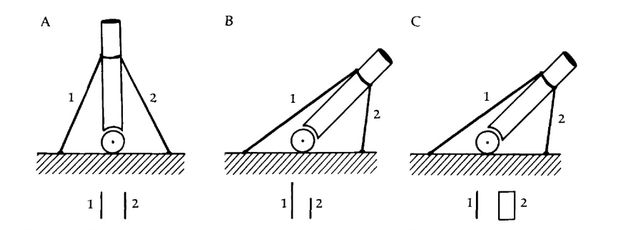
\includegraphics[width=70mm]{figs/l9/spring.png}
\end{center}

\begin{itemize}
 \item rubber band of equal or unequal length
 \item increasing or decreasing length of muscles
 \item increasing or decreasing stiffness of muscles 
 \item[$\rightarrow$] compute position and translate into muscle length or stiffness
\end{itemize}
\end{overlayarea}
\end{frame}


\begin{frame}
 \frametitle{Summary}
\begin{itemize}
\setlength{\itemsep}{5pt}
 \item hand movements already in utero, by months 9 reliable control of direction and distance of reach and grasp
 \item use of visual feedback susceptible to experience
 \item vision dominates touch
 \item vision for action may use different neural subsystem than vision for recognition
 \item eye and hand are tightly coupled in visually guided manual aiming tasks
 \item amplitude errors tend to be larger than direction errors
 \item speed profiles scale with distance to be covered
 \item Fitts' law provides an accurate description of the relationship between target width, distance and 
\end{itemize}
\end{frame}



\begin{frame}
 \frametitle{References}
\begin{small}
\begin{itemize}
 \item  Wolfe, J.M., Kluender, K.R. \& Levi, D.M. (2012).\textit{Sensation \& Perception}. Sinauer Associates: Sunderland, MA. 
\end{itemize}
\end{small}
\end{frame}


\end{document}